
\begin{figure}

\centering

\tikzset{every picture/.style={line width=0.75pt}} %set default line width to 0.75pt        

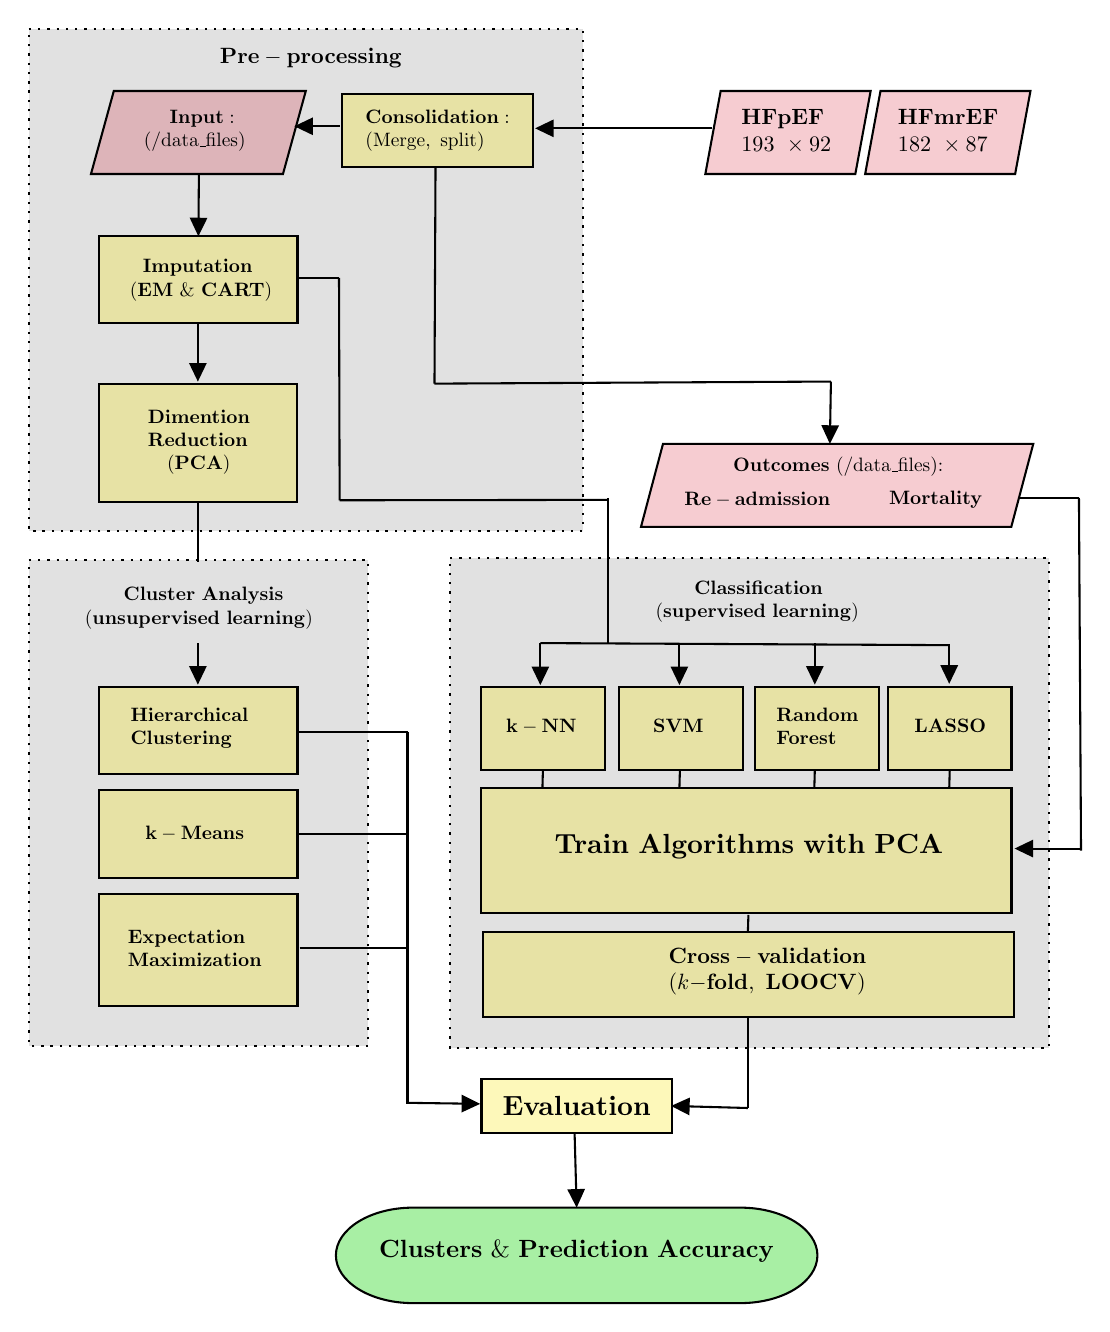
\begin{tikzpicture}[x=0.75pt,y=0.75pt,yscale=-1,xscale=1]
%uncomment if require: \path (0,646); %set diagram left start at 0, and has height of 646

%Shape: Rectangle
\draw  [fill={rgb, 255:red, 155; green, 155; blue, 155 }  ,fill opacity=0.3 ][dash pattern={on 0.84pt off 2.51pt}] (2,5) -- (269,5) -- (269,247) -- (2,247) -- cycle ;
%Shape: Rectangle
\draw  [fill={rgb, 255:red, 155; green, 155; blue, 155 }  ,fill opacity=0.3 ][dash pattern={on 0.84pt off 2.51pt}] (205,260) -- (493.5,260) -- (493.5,496) -- (205,496) -- cycle ;
%Shape: Rectangle
\draw  [fill={rgb, 255:red, 155; green, 155; blue, 155 }  ,fill opacity=0.3 ][dash pattern={on 0.84pt off 2.51pt}] (2,261) -- (165.5,261) -- (165.5,495) -- (2,495) -- cycle ;
%Straight Lines
\draw    (84,75) -- (83.77,103) ;
\draw [shift={(83.75,105)}, rotate = 270.48] [fill={rgb, 255:red, 0; green, 0; blue, 0 }  ][line width=0.75]  [draw opacity=0] (8.93,-4.29) -- (0,0) -- (8.93,4.29) -- cycle    ;

%Straight Lines
\draw    (83.5,147) -- (83.5,173) ;
\draw [shift={(83.5,175)}, rotate = 270] [fill={rgb, 255:red, 0; green, 0; blue, 0 }  ][line width=0.75]  [draw opacity=0] (8.93,-4.29) -- (0,0) -- (8.93,4.29) -- cycle    ;

%Straight Lines
\draw    (184.5,344) -- (184.5,523) ;


%Straight Lines
\draw    (184.5,522.5) -- (217.5,522.97) ;
\draw [shift={(219.5,523)}, rotate = 180.82] [fill={rgb, 255:red, 0; green, 0; blue, 0 }  ][line width=0.75]  [draw opacity=0] (8.93,-4.29) -- (0,0) -- (8.93,4.29) -- cycle    ;

%Straight Lines
\draw    (248.5,301) -- (248.5,319.22) ;
\draw [shift={(248.5,321.22)}, rotate = 270] [fill={rgb, 255:red, 0; green, 0; blue, 0 }  ][line width=0.75]  [draw opacity=0] (8.93,-4.29) -- (0,0) -- (8.93,4.29) -- cycle    ;

%Straight Lines
\draw    (315.5,301) -- (315.5,319.22) ;
\draw [shift={(315.5,321.22)}, rotate = 270] [fill={rgb, 255:red, 0; green, 0; blue, 0 }  ][line width=0.75]  [draw opacity=0] (8.93,-4.29) -- (0,0) -- (8.93,4.29) -- cycle    ;

%Straight Lines
\draw    (380.75,301) -- (380.75,319) ;
\draw [shift={(380.75,321)}, rotate = 270] [fill={rgb, 255:red, 0; green, 0; blue, 0 }  ][line width=0.75]  [draw opacity=0] (8.93,-4.29) -- (0,0) -- (8.93,4.29) -- cycle    ;

%Straight Lines
\draw    (445.5,301.39) -- (445.5,318.61) ;
\draw [shift={(445.5,320.61)}, rotate = 270] [fill={rgb, 255:red, 0; green, 0; blue, 0 }  ][line width=0.75]  [draw opacity=0] (8.93,-4.29) -- (0,0) -- (8.93,4.29) -- cycle    ;

%Straight Lines
\draw    (248.5,301) -- (445.5,302) ;


%Straight Lines
\draw    (348.5,481) -- (348.5,525) ;


%Straight Lines
\draw    (313.5,524.05) -- (348.5,525) ;

\draw [shift={(311.5,524)}, rotate = 1.55] [fill={rgb, 255:red, 0; green, 0; blue, 0 }  ][line width=0.75]  [draw opacity=0] (8.93,-4.29) -- (0,0) -- (8.93,4.29) -- cycle    ;
%Shape: Rectangle
\draw  [fill={rgb, 255:red, 248; green, 231; blue, 28 }  ,fill opacity=0.3 ] (220,371) -- (475.5,371) -- (475.5,431) -- (220,431) -- cycle ;
%Straight Lines
\draw    (281,231) -- (281,301) ;


%Straight Lines
\draw    (479,231) -- (508,231) ;


%Straight Lines
\draw    (508,231) -- (509,401) ;


%Straight Lines
\draw    (479,400) -- (509,400) ;

\draw [shift={(477,400)}, rotate = 0] [fill={rgb, 255:red, 0; green, 0; blue, 0 }  ][line width=0.75]  [draw opacity=0] (8.93,-4.29) -- (0,0) -- (8.93,4.29) -- cycle    ;
%Shape: Rectangle
\draw  [fill={rgb, 255:red, 248; green, 231; blue, 28 }  ,fill opacity=0.3 ] (36,105) -- (131.5,105) -- (131.5,147) -- (36,147) -- cycle ;
%Shape: Rectangle
\draw  [fill={rgb, 255:red, 248; green, 231; blue, 28 }  ,fill opacity=0.3 ] (35.75,176) -- (131.25,176) -- (131.25,233) -- (35.75,233) -- cycle ;
%Shape: Rectangle
\draw  [fill={rgb, 255:red, 248; green, 231; blue, 28 }  ,fill opacity=0.3 ] (36,322) -- (131.5,322) -- (131.5,364) -- (36,364) -- cycle ;
%Shape: Rectangle
\draw  [fill={rgb, 255:red, 248; green, 231; blue, 28 }  ,fill opacity=0.3 ] (36,372) -- (131.5,372) -- (131.5,414) -- (36,414) -- cycle ;
%Shape: Rectangle
\draw  [fill={rgb, 255:red, 248; green, 231; blue, 28 }  ,fill opacity=0.3 ] (36,422) -- (131.5,422) -- (131.5,476) -- (36,476) -- cycle ;
%Straight Lines
\draw    (131.5,344) -- (184.5,344) ;


%Straight Lines
\draw    (131.5,393) -- (184.5,393) ;


%Straight Lines
\draw    (132.5,448) -- (184.5,448) ;


%Straight Lines
\draw    (151.8,232.2) -- (281,232) ;


%Straight Lines
\draw    (151.5,125) -- (151.8,232.2) ;


%Straight Lines
\draw    (131.5,125) -- (151.5,125) ;


%Shape: Rectangle
\draw  [fill={rgb, 255:red, 248; green, 231; blue, 28 }  ,fill opacity=0.3 ] (220,322) -- (279.5,322) -- (279.5,362) -- (220,362) -- cycle ;
%Shape: Rectangle
\draw  [fill={rgb, 255:red, 248; green, 231; blue, 28 }  ,fill opacity=0.3 ] (286.5,322) -- (346,322) -- (346,362) -- (286.5,362) -- cycle ;
%Shape: Rectangle
\draw  [fill={rgb, 255:red, 248; green, 231; blue, 28 }  ,fill opacity=0.3 ] (352,322) -- (411.5,322) -- (411.5,362) -- (352,362) -- cycle ;
%Shape: Rectangle
\draw  [fill={rgb, 255:red, 248; green, 231; blue, 28 }  ,fill opacity=0.3 ] (416,322) -- (475.5,322) -- (475.5,362) -- (416,362) -- cycle ;
%Straight Lines
\draw    (249.5,371) -- (249.75,362) ;


%Straight Lines
\draw    (315.5,371) -- (315.75,362) ;


%Straight Lines
\draw    (380.5,371) -- (380.75,362) ;


%Straight Lines
\draw    (445.5,371) -- (445.75,362) ;


%Shape: Rectangle
\draw  [fill={rgb, 255:red, 248; green, 231; blue, 28 }  ,fill opacity=0.3 ] (221,440) -- (476.5,440) -- (476.5,481) -- (221,481) -- cycle ;
%Straight Lines
\draw    (83.5,233) -- (83.5,262) ;


%Straight Lines
\draw    (348.5,440) -- (348.75,432) ;


%Straight Lines
\draw    (265,537) -- (265.94,571) ;
\draw [shift={(266,573)}, rotate = 268.40999999999997] [fill={rgb, 255:red, 0; green, 0; blue, 0 }  ][line width=0.75]  [draw opacity=0] (8.93,-4.29) -- (0,0) -- (8.93,4.29) -- cycle    ;

%Shape: Parallelogram
\draw  [fill={rgb, 255:red, 208; green, 2; blue, 27 }  ,fill opacity=0.2 ] (335.38,35) -- (407.64,35) -- (400.26,75) -- (328,75) -- cycle ;
%Straight Lines
\draw    (83.5,301) -- (83.5,319) ;
\draw [shift={(83.5,321)}, rotate = 270] [fill={rgb, 255:red, 0; green, 0; blue, 0 }  ][line width=0.75]  [draw opacity=0] (8.93,-4.29) -- (0,0) -- (8.93,4.29) -- cycle    ;

%Straight Lines
\draw    (197.5,176) -- (388.5,175) ;


%Straight Lines
\draw    (388.5,175) -- (388.03,203) ;
\draw [shift={(388,205)}, rotate = 270.95] [fill={rgb, 255:red, 0; green, 0; blue, 0 }  ][line width=0.75]  [draw opacity=0] (8.93,-4.29) -- (0,0) -- (8.93,4.29) -- cycle    ;

%Straight Lines
\draw    (197.5,176) -- (198,72) ;


%Straight Lines
\draw    (132,52) -- (152,52) ;

\draw [shift={(130,52)}, rotate = 0] [fill={rgb, 255:red, 0; green, 0; blue, 0 }  ][line width=0.75]  [draw opacity=0] (8.93,-4.29) -- (0,0) -- (8.93,4.29) -- cycle    ;
%Straight Lines
\draw    (248,53) -- (331,53) ;

\draw [shift={(246,53)}, rotate = 0] [fill={rgb, 255:red, 0; green, 0; blue, 0 }  ][line width=0.75]  [draw opacity=0] (8.93,-4.29) -- (0,0) -- (8.93,4.29) -- cycle    ;
%Shape: Parallelogram
\draw  [fill={rgb, 255:red, 208; green, 2; blue, 27 }  ,fill opacity=0.2 ] (43,35) -- (135.5,35) -- (124.5,75) -- (32,75) -- cycle ;
%Shape: Parallelogram
\draw  [fill={rgb, 255:red, 208; green, 2; blue, 27 }  ,fill opacity=0.2 ] (307.6,205) -- (486,205) -- (475.4,245) -- (297,245) -- cycle ;
%Shape: Parallelogram
\draw  [fill={rgb, 255:red, 208; green, 2; blue, 27 }  ,fill opacity=0.2 ] (412.38,35) -- (484.64,35) -- (477.26,75) -- (405,75) -- cycle ;
%Flowchart: Terminator
\draw  [fill={rgb, 255:red, 139; green, 233; blue, 134 }  ,fill opacity=0.75 ] (187.12,573) -- (344.88,573) .. controls (365.38,573) and (382,583.3) .. (382,596) .. controls (382,608.7) and (365.38,619) .. (344.88,619) -- (187.12,619) .. controls (166.62,619) and (150,608.7) .. (150,596) .. controls (150,583.3) and (166.62,573) .. (187.12,573) -- cycle ;

% Text Node
\draw (82,54) node [scale=0.7]  {$ \begin{array}{l}
\ \ \ \ \mathbf{Input:}\\
( /\mathrm{data\_files})
\end{array}$};
% Text Node
\draw (85,126) node [scale=0.7]  {$ \begin{array}{l}
\ \ \mathbf{Imputation}\\
\mathbf{( EM\ \&\ CART)}
\end{array}$};
% Text Node
\draw (84,204) node [scale=0.7]  {$ \begin{array}{l}
\mathbf{Dimention}\\
\mathbf{Reduction}\\
\ \ \ \mathbf{( PCA)}
\end{array}$};
% Text Node
\draw (81,342) node [scale=0.7]  {$ \begin{array}{l}
\mathbf{Hierarchical\ }\\
\mathbf{Clustering}
\end{array}$};
% Text Node
\draw (82,393) node [scale=0.7]  {$\mathbf{k-Means}$};
% Text Node
\draw (82,449) node [scale=0.7]  {$ \begin{array}{l}
\mathbf{Expectation}\\
\mathbf{Maximization}
\end{array}$};
% Text Node
\draw (84,284) node [scale=0.7]  {$ \begin{array}{l}
\ \ \ \ \ \ \mathbf{Cluster\ Analysis}\\
\mathbf{( unsupervised\ learning)}
\end{array}$};
% Text Node
\draw  [fill={rgb, 255:red, 248; green, 231; blue, 28 }  ,fill opacity=0.3 ]  (220.16,511) -- (311.84,511) -- (311.84,537) -- (220.16,537) -- cycle  ;
\draw (266,524) node   {$\mathbf{Evaluation}$};
% Text Node
\draw (249,341) node [scale=0.7]  {$\mathbf{k-NN}$};
% Text Node
\draw (315,341) node [scale=0.7]  {$\mathbf{SVM}$};
% Text Node
\draw (382,342) node [scale=0.7]  {$ \begin{array}{l}
\mathbf{Random}\\
\mathbf{Forest}
\end{array}$};
% Text Node
\draw (446,341) node [scale=0.7]  {$\mathbf{LASSO}$};
% Text Node
\draw (349,459) node [scale=0.8]  {$ \begin{array}{l}
\ \ \ \ \ \mathbf{Cross-validation}\\
\ \ \ \ \ \mathbf{(} k\mathbf{-fold} ,\ \mathbf{LOOCV)}
\end{array}$};
% Text Node
\draw (353,281) node [scale=0.7]  {$ \begin{array}{l}
\ \ \ \ \ \ \mathbf{Classification}\\
\mathbf{( supervised\ learning)}
\end{array}$};
% Text Node
\draw (349,399) node   {$\mathbf{Train\ Algorithms\ with\ PCA}$};
% Text Node
\draw (266,594) node [scale=0.9]  {$\mathbf{Clusters\ \&\ Prediction\ Accuracy}$};
% Text Node
\draw (353,232) node [scale=0.7]  {$\mathbf{Re-admission}$};
% Text Node
\draw (439,232) node [scale=0.7]  {$\mathbf{Mortality}$};
% Text Node
\draw (392,216) node [scale=0.7]  {$\mathbf{Outcomes\ (} /\mathrm{data\_files})\mathbf{:}$};
% Text Node
\draw (445,55) node [scale=0.8]  {$ \begin{array}{l}
\mathbf{HFmrEF}\\
182\ \times 87
\end{array}$};
% Text Node
\draw (367,55) node [scale=0.8]  {$ \begin{array}{l}
\mathbf{HFpEF}\\
193\ \times 92
\end{array}$};
% Text Node
\draw  [fill={rgb, 255:red, 248; green, 231; blue, 28 }  ,fill opacity=0.3 ]  (153.05,36.5) -- (244.95,36.5) -- (244.95,71.5) -- (153.05,71.5) -- cycle  ;
\draw (199,54) node [scale=0.7]  {$ \begin{array}{l}
\mathbf{Consolidation} :\\
(\mathrm{Merge,\ split})
\end{array}$};
% Text Node
\draw (138,19) node [scale=0.8]  {$\mathbf{Pre-processing}$};

\end{tikzpicture}



\caption[Machine learning procedure adopted in the thesis]{\textit{Machine learning procedure adopted in the thesis}}
\label{fig:ML_proc_thesis}
\normalsize
\end{figure}